\documentclass[a4paper]{article}
\usepackage[usenames,dvipsnames]{xcolor}
\usepackage{caption}
\usepackage{amsmath}
\usepackage{amsfonts}
\usepackage{amssymb}
\usepackage{subcaption}
\usepackage{listings}
\usepackage{qtree}
\usepackage{xcolor}
\usepackage{forest}
\usepackage{multicol}
\setlength{\columnsep}{3cm}
\usepackage{parskip}
\usepackage{changepage}
\usepackage[T1]{fontenc}
\usepackage{amsmath}
\usepackage{hyperref}
\usepackage{listings}
\usepackage{amsthm}
\usepackage{amssymb}
\usepackage{float}
\usepackage[utf8]{inputenc}
\usepackage{graphicx}
\usepackage[italian]{babel}
\usepackage{thmtools}
\usepackage{mathtools}
\newtheorem*{definition}{Def}
\usepackage{xcolor}
\newcommand{\appunto}[1]{\textcolor{ForestGreen}{#1}}
\newcommand{\E}[0]{\mathbb{E}}
\renewcommand{\thesubsection}{\thesection.\alph{subsection}}


\begin{document}

\author{Giulia Coucorde 802321 giulia.coucourde@edu.unito.it,\\ Andrea Cacioli 914501 andrea.cacioli@edu.unito.it,\\ Lorenzo Dentis 914833 lorenzo.dentis@edu.unito.it}
\title{Risposte Foglio1}
\maketitle
\section{Esercizio 1}
Si consideri una catena di Markov con matrice di transizione.
$$P=\left(\begin{array}{c c c}{{\frac{1}{2}}}&{{\frac{1}{3}}}&{{\frac{1}{4}}}\\ {{\frac{3}{4}}}&{{0}}&{{\frac{1}{4}}}\\ {{0}}&{{1}}&{{0}}\end{array}\right)$$
\begin{itemize}
	\item Stabilire se sia una catena irreducibile.\\
	Una catena si dice irreducibile quando presenta una sola classe di equivalenza rispetto alla relazione \textit{comunicazione}.
		Si dimostra facilmente che $P$ è irreducibile disegnando il suo grafo pesato:\\
		\begin{center}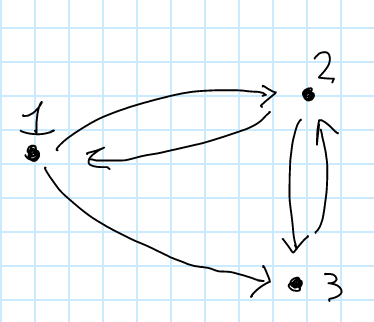
\includegraphics[scale=0.3]{grafo.png}\end{center}
		Dal disegno si nota facilmente che ${1,2,3}$ è l'unica classe di equivalenza della catena, $(1,2)$ e $(2,3)$ comunicano direttamente, la coppia $(1,3)$ comunica grazie alla transitività della relazione \textit{comunicazione}.\\
		$ 1 \rightarrow 3$ è una relazione di comunicazione diretta e $3 \rightarrow 2 \land 2 \rightarrow 1 \Rightarrow 3 \rightarrow 1$ 
	\item Supponendo che il processo sia originato nello stato 1, determinare la probabilitá che si trovi nello stato 3 dopo due passi\\
		Per trovare la probabilità che un sistema si trovi in un dato stato basta utilizzare la matrice di transizione, come dimostrato a lezione se si vuole considerare l'evoluzione dopo $n$ passi basta considerare la matrice di transizione $P^n$. In questo caso ci interessa $P^2$.\\
		$$P^2=P*P= \left(\begin{array}{c c c}{{\frac{1}{2}}}&{{\frac{1}{3}}}&{{\frac{1}{4}}}\\ {{\frac{3}{4}}}&{{0}}&{{\frac{1}{4}}}\\ {{0}}&{{1}}&{{0}}\end{array}\right) *
		\left(\begin{array}{c c c}{{\frac{1}{2}}}&{{\frac{1}{3}}}&{{\frac{1}{4}}}\\ {{\frac{3}{4}}}&{{0}}&{{\frac{1}{4}}}\\ {{0}}&{{1}}&{{0}}\end{array}\right)
		= \left(\begin{array}{c c c}{{\frac{1}{2}}}&{{\frac{1}{3}}}&{{\frac{1}{6}}}\\ {{\frac{3}{8}}}&{{\frac{1}{2}}}&{{\frac{1}{8}}}\\ {{\frac{3}{4}}}&{{0}}&{{\frac{1}{4}}}\end{array}\right) $$
	\item Determinare $lim_{n \rightarrow \infty}P^n$
		Per ottenere la distribuzione limite possiamo utilizzare il teorema presentato in classe. La catena $P$ è irreducibile (dimostrato al punto 1) ed Ergodica, questo perchè tutti gli stati sono aperiodici e la catena è irreducibile, quindi sappiamo:
		\begin{enumerate}
			\item esiste $lim_{n \rightarrow \infty}P^n_{ij}=\Pi_j$
			\item $\Pi_j$ è l'unica soluzione del seguente sistema: 
				\begin{equation*}
					\begin{cases} \Pi_j = \sum_i \Pi_j P_{ij}\\
						\sum \Pi_j = 1
					\end{cases}
				\end{equation*}
		\end{enumerate}
		Aplicandolo al nostro caso ottieniamo il seguente sistema:
		\begin{align*}
			\begin{cases}
				\frac{1}{2}\Pi_1 * \frac{3}{4}\Pi_2 * 0\Pi_3 = \Pi\\
				\frac{1}{3}\Pi_1 * 0\Pi_2 * 1\Pi_3 = \Pi\\
				\frac{1}{6}\Pi_1 * \frac{1}{4}\Pi_2 * 0\Pi_3 = \Pi\\
				\Pi_1 + \Pi_2 + \Pi_3 = 1
			\end{cases}
			= \textit{ risolvendo } = 
			\begin{cases}
				\Pi_1 = \frac{1}{2}\\
				\Pi_2 = \frac{1}{3}\\
				\Pi_3 = \frac{1}{6}
			\end{cases}
		\end{align*}
\end{itemize}
\section{Esercizio 4}
Si considerino due distinte code di tipo M/M/1 (code in cui i clienti arrivino secondo un processo di Poisson e vengano serviti da un unico servitore con tempi di servizio esponenziali).
Si supponga che nella prima coda il processo di Poisson abbia parametro $\lambda_1$ , mentre nella seconda abbia parametro $\lambda_2$ ; inoltre il tempo di servizio sia analogo per le due code, con tempo medio di servizio $\mu$. Si supponga $\lambda_1 < \lambda_2 < \mu$
\subsection{}
Si puó affermare che in ogni istante ci saranno sicuramente meno clienti in attesa nella prima coda?
No, non lo si può affermare, in quanto si possono trovare 3 controesempi:\\
Il primo controesempio è la situazione in cui non c'è alcun cliente in coda ed arriva un cliente prima prima coda che nella seconda, cosa comunque possibile nonostante $\lambda_1 < \lambda_2$.\\
Più interessante è la situazione in cui entrambe le code hanno $n$ clienti. 
\begin{center}\makebox[0cm]{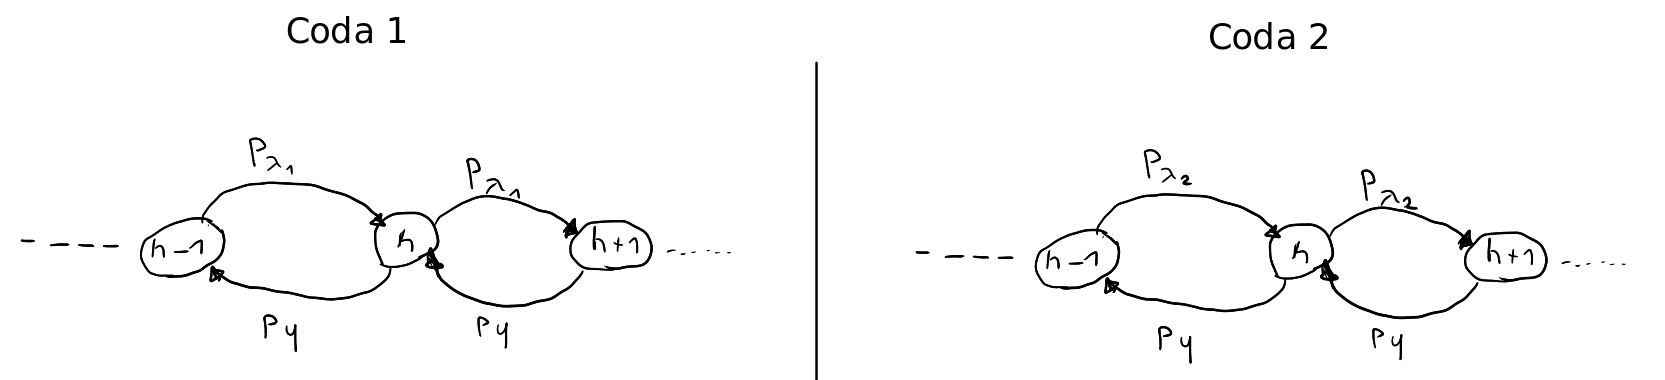
\includegraphics[scale=0.3]{code.png}}\end{center}
In questo caso ci sono due situazioni in cui la prima coda ha più clienti in attesa della seconda, se un cliente arriva nella coda 1 ($P_{\lambda_1}$), o se un cliente esce dalla coda 2 ($P_\mu$).
\subsection{}
Si puó affermare che in media ci saranno meno clienti nella coda 1? Giustificare la risposta.
Si, in media ci saranno meno clienti nella prima coda. Tra le proprietà della coda M|M|1 vi è una proprietà che, sotto la condizione $\lambda < \mu$, permette di calcolare il numero medio di persone in coda.
\begin{align*}
	&\text{posto } \lambda < \mu \text{ e creando un nuovo parametro } \rho = \frac{\lambda}{\mu} \\
	&\text{Il numero medio di utenti in coda è } L_{q}=\sum_{k=1}^{\infty}{(k-1)\pi_{i}}=\frac{\rho^{2}}{1-\rho}
\end{align*}
Nel caso dell'esercizio $\lambda_1 < \lambda_2$ e $\mu$ uguale per le due code quindi\\ $\rho_1 = \frac{\lambda_1}{\mu} < \rho_2 = \frac{\lambda_2}{\mu}$
$$L_{q1} = \frac{\rho_1^{2}}{1-\rho_1} < L_{q2} = \frac{\rho_2^{2}}{1-\rho_2}$$
Si può quindi affermare che in media la coda 2 avrà più clienti della coda 1.
\end{document}
